\begin{exercício}{}{exercício2}
    O princípio ativo do colorante Cl 42555 (violeta crista) é o cátion orgânico monovalente \ce{C[C6H4N(CH3)2]3^+}. O esqueleto desse íon é constituído por três ramos idênticos, como na figura abaixo, o déficit eletrônico responsável pela carga \(+\) podendo ter sido retirado de qualquer um dos três ramos.
    \begin{center}
        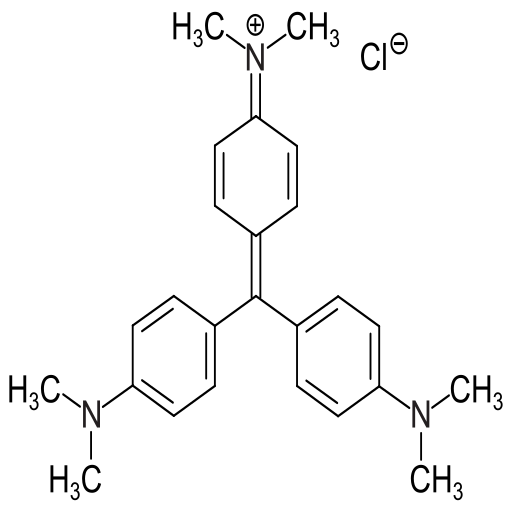
\includegraphics[height=0.15\textheight]{Cl42555.png}
    \end{center}
    Podemos tratar o estado eletrônico desse íon como um sistema de três estados. O hamiltoniano \(H\) não é diagonal na base ortonormal \(\set{\ket{1},\ket{2}, \ket{3}}\) correspondente aos estados das \enquote{configurações clássicas}, pois é possível passar de uma \enquote{configuração clássica} para outra por um efeito quântico denominado efeito túnel que estudaremos futuramente.
    \begin{enumerate}[label=(\alph*)]
        \item Trabalharemos na base de \enquote{configurações clássicas}. Escolheremos a origem das energias tal que tenhamos \(\bra{n}H\ket{n} = 0.\) Temos também \(\bra{1}H\ket{2} = \bra{2}H\ket{3} = \bra{3}H\ket{1} = -A,\) onde \(A > 0\). Escreva a matriz que representa \(H\) nessa base.
        \item Considere os estados \(\ket{\phi_1} = \frac{1}{\sqrt{3}} (\ket{1} + \ket{2} + \ket{3})\) e \(\ket{\phi_2} = \frac1{\sqrt{2}} (\ket{2} - \ket{3}\). Calcule o valor médio da energia e seu desvio padrão para cada um desses estados.
        \item Determine os níveis de energia do sistema. Encontre uma base ortonormal simples. Essa base é única?
    \item Temos \(A \sim \SI{0.75}{eV}.\) Por que o íon tem cor violeta? Lembramos que as cores do espectro da luz branca são, em ordem de energia crescente:
        \begin{enumerate}[label=(\roman*)]
            \item vermelho \(\SI{1.65}{eV} \sim \SI{2.0}{eV}\);
            \item laranja \(\SI{2.0}{eV} \sim \SI{2.1}{eV}\);
            \item amarelo \(\SI{2.1}{eV} \sim \SI{2.3}{eV}\);
            \item verde \(\SI{2.3}{eV} \sim \SI{2.55}{eV}\);
            \item azul \(\SI{2.55}{eV} \sim \SI{2.65}{eV}\); e
            \item violeta \(\SI{2.65}{eV} \sim \SI{3.1}{eV}\).
        \end{enumerate}
        As pares principais de \enquote{cores complementares} que associadas restituem a luz branca são amarelo-violeta, vermelho-verde e azul-laranja.
    \item Substituímos o grupo \ce{N(CH3)2} do ramo superior por um átomo de hidrogênio. Supomos que o único efeito dessa substituição seja de elevar \(\bra{1}H\ket{1}\) de uma certa quantidade \(\Delta > 0\), deixando os outros elementos de \(H\) inalterados. Mostre que \(A\) continua autovalor do hamiltoniano. Quais os outros níveis de energia do novo sistema? O que acontece nos limites \(\Delta \ll A\) e \(\Delta \gg A\)?
    \item Esse íon modificado (colorante Cl 42000, verde de malaquita) absorve em dois comprimentos de onda: \SI{620}{nm} e \SI{450}{nm}. Calcule \(\Delta\) e comente sobre concordância entre teoria e experiência.
    \end{enumerate}
\end{exercício}
\begin{proof}[Resolução]
    Na base de configurações clássicas temos
    \begin{equation*}
        H = \begin{pmatrix}
            0 &&-A &&-A\\
            -A&& 0 &&-A\\
            -A&& -A&&0
        \end{pmatrix}
    \end{equation*}
    como a representação do hamiltoniano \(H\). Notemos que
    \begin{align*}
        H\ket{\phi_1} = -2A\ket{\phi_1}\quad\text{e}\quad
        H\ket{\phi_2} = A\ket{\phi_2},
    \end{align*}
    portanto os estados \(\ket{\phi_1}\) e \(\ket{\phi_2}\) são autovetores do hamiltoniano correspondente aos autovalores \(-2A\) e \(A\), respectivamente. Assim, nesses estados, os valores médios de energia são justamente esses autovalores, com desvio padrão nulo.

    Para completar a base de autoestados, consideremos \(\ket{\phi} = \frac1{\sqrt{2}}\left(\ket{1} - \ket{3}\right)\), então \(H\ket{\phi} = A\ket{\phi}\) com \(\set{\ket{\phi_2}, \ket{\phi}}\) linearmente independente, portanto os níveis de energia são \(-2A\) e \(A\). Aplicando o método de Gram-Schmidt nesta base do autoespaço associado à energia \(A\), segue que \(\set{\ket{\phi_1}, \ket{\phi_2}, \ket{\phi_3}}\) é uma base ortonormal com \(\ket{\phi_3} = \frac{1}{\sqrt{6}}\left(2\ket{1} - \ket{2} - \ket{3}\right)\). Notemos ainda que essa base não é única pois qualquer operador unitário \(U\) com \(\ket{\phi_1}\) como autovetor leva esta base a uma outra base de autoestados ortogonais.

    Quando luz branca incide no íon, os comprimentos de onda associados ao amarelo, de energia \(3A \sim \SI{2.25}{eV}\), são capazes de mudar o nível de energia de \(-2A\) para \(A\). Assim, o íon absorve esta parte do espectro, e a luz refletida contém o restante do espectro, resultando na cor complementar violeta, uma vez que o restante do espectro restitui a luz branca.

    Substituindo o grupo \ce{N(CH3)2} do ramo superior por um átomo de hidrogênio,
    \begin{equation*}
        \tilde{H} = \begin{pmatrix}
            \Delta &&-A &&-A\\
            -A&& 0 &&-A\\
            -A&& -A&&0
        \end{pmatrix}
    \end{equation*}
    é a representação do hamiltoniano para este íon modificado na base de configurações clássicas. Assim, o polinômio característico de \(\tilde{H}\) é dado por
    \begin{align*}
        p_{\tilde{H}}(\lambda) = \det(\tilde{H} - \lambda \unity) &= \lambda (A - \lambda) (\Delta + A - \lambda) + A (2 \lambda - 2A - \Delta)(\lambda - A)\\
                                                                  &= (A - \lambda)(\Delta\lambda + A \lambda - \lambda^2 - 2A \lambda + 2A^2 + A \Delta)\\
                                                                  &= (\lambda - A)[\lambda^2 - (\Delta - A)\lambda - (2A^2 + A \Delta)]\\
                                                                  &= (\lambda - A)(\lambda - A_+)(\lambda - A_-),
    \end{align*}
    onde
    \begin{equation*}
        A_{\pm} = \frac{\Delta - A \pm \sqrt{\Delta^2 + 2A \Delta + 9A^2}}{2}.
    \end{equation*}
    Desta forma, o espectro do hamiltoniano para o íon modificado é \(\set{A, A_-, A_+}\). Notemos que para \(\Delta \gg A\), temos
    \begin{equation*}
        A_\pm = \Delta \frac{1 - \frac{A}{\Delta} \pm \sqrt{1 + 2\frac{A}{\Delta} + 9\left(\frac{A}{\Delta}\right)^2}}{2} = \frac{\Delta - A \pm (\Delta + A)}{2} + O\left[\left(\frac{A}{\Delta}\right)^2\right],
    \end{equation*}
    portanto o espectro se aproxima de \(\set{A, -A, \Delta}\). No caso em que \(\Delta \ll A\), temos
    \begin{equation*}
        A_{\pm} = A\frac{\frac{\Delta}{A} - 1 \pm 3\sqrt{\left(\frac{\Delta}{3A}\right)^2 + 2\frac{\Delta}{9A} + 1}}{2} = \frac{\Delta - A \pm (3A + \frac{\Delta}{3})}{2} + O\left[\left(\frac{\Delta}{A}\right)^2\right],
    \end{equation*}
    logo o espectro se aproxima de \(\set{A, \frac{2 \Delta}{3} + A, -2A + \frac{\Delta}{3}}\).

    Se o íon modificado absorve nos comprimentos de \SI{620}{nm} e de \SI{450}{nm}, segue que as diferenças entre os níveis de energia correspondentes às absorções são \SI{2.00}{eV} e \SI{2.76}{eV}, isto é, \(\sim \frac{8}{3}A\) e \(\sim \frac{11}{3}A\). Notemos que estas diferenças
    não se adéquam aos casos \(\Delta \gg A\) ou \(\Delta \ll A\). No caso geral, temos \(A_- < A < A_+\), com
    \begin{equation*}
        A_+ - A = \frac{3A - \Delta - \sqrt{\Delta^2 + 2A \Delta + 9A^2}}{2} \quad\text{e}\quad
        A_+ - A_- = \sqrt{\Delta^2 + 2A \Delta + 9A^2}.
    \end{equation*}
    Assim, temos \(A_+ - A_- = \frac{11}{3}A\) e \(A_+ - A = \frac83A\), donde segue que
    \begin{equation*}
        \frac{8}{3}A = \frac{3A - \Delta - \frac{11}{3}A}{2} \implies \Delta = - 6A,
    \end{equation*}
    o que não é possível, pois por hipótese \(\Delta > 0\). Concluímos que o hamiltoniano \(\tilde{H}\) não é um modelo adequado para o íon modificado.
\end{proof}
